\subsection{Schraubenfeder \hfill ME}
    \begin{center}
        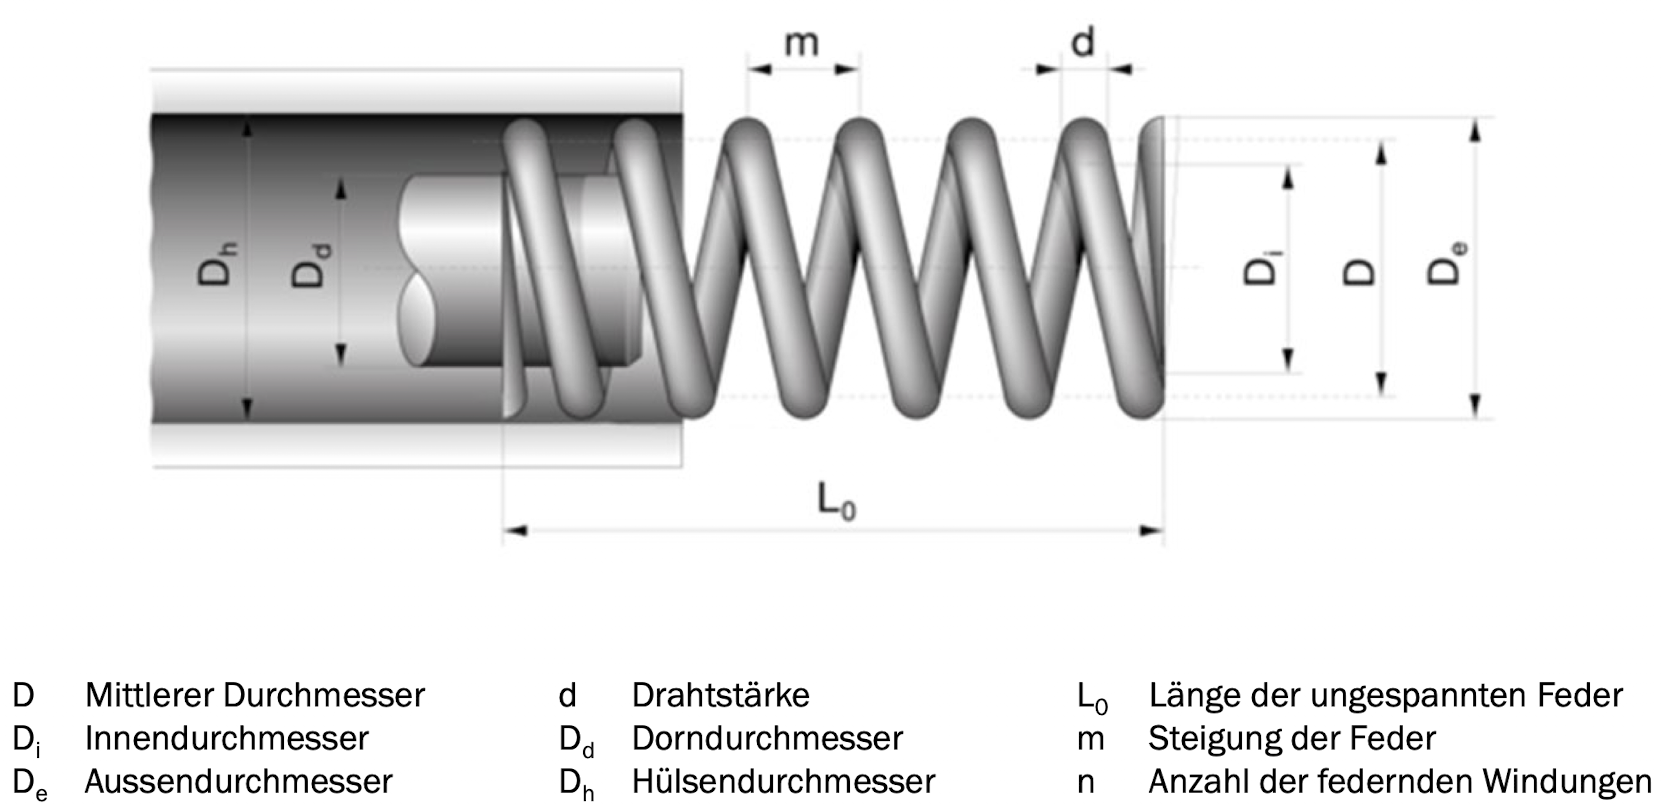
\includegraphics[width = 0.8\linewidth]{src/images/MAEIP_Schraubenfeder}

    \end{center}
    \begin{minipage}{0.57\linewidth}
        \begin{footnotesize}
            \begin{empheq}[box = \fbox]{align*}
                R &= \frac{G \cdot d^4}{8 \cdot D^3 \cdot n}
                \\F &= R \cdot s
                \\W &= \frac{1}{2} \cdot R (s_2^2 -s_1^2) \: [\text{Nmm}]
                \\ &= \frac{1}{2} \cdot (F_2s_2 - F_1s_1)
                \\\tau_t &= G \cdot tan(\gamma)
                \\ D&= D_e -d
            \end{empheq}
        \end{footnotesize}
    \end{minipage}
    \begin{minipage}{0.41\linewidth}
        \begin{scriptsize}
            \begin{empheq}[box= \fbox]{align*}
                R &= \text{Federrate}
                \\ G&= \text{Schubmodul}
                \\ \tau_t &= \text{Torsionsspannung}
                \\W &= \text{Federarbeit}
                \\\gamma &= \text{Verdrehwinkel}
                \\ n &= \text{\# federnde Windungen}
            \end{empheq}
        \end{scriptsize}
    \end{minipage}